% Preamble
\documentclass[11pt,parskip=half-]{scrartcl}

\usepackage{lmodern}
\usepackage[british]{babel}
\usepackage{minted}
\usepackage{ugent2016-assets}
\usepackage{graphicx}
\usepackage{array}
\usepackage{textcomp}
\usepackage{hologo}
\usepackage[colorlinks]{hyperref}
\usepackage{sidenotes}
\usepackage{enumitem}
\usepackage{fontspec}
\usepackage[Q=yes]{examplep}
\usepackage{multicol}
\usepackage{titling}

\title{Packages for documents in Ghent University style}
\author{Niko Strijbol}

\setcounter{tocdepth}{2}

% customize dictum format:
\setkomafont{dictumtext}{\itshape\small}
\setkomafont{dictumauthor}{\normalfont}
\renewcommand*\dictumwidth{\linewidth}
\renewcommand*\dictumauthorformat[1]{--- #1}
\renewcommand*\dictumrule{}

\newcommand*{\LuaLaTeX}{\hologo{LuaLaTeX}}

\BeforeStartingTOC[toc]{\begin{multicols}{2}}
\AfterStartingTOC[toc]{\end{multicols}}

\usepackage[bottom=3cm,top=2cm]{geometry}

% Document
\begin{document}
    \maketitle

    \begin{abstract}
        \noindent This bundle contains some packages and classes to give \LaTeX\ the possibility to create reports, articles and books that comply with the official corporate style of Ghent University.
    \end{abstract}

    \tableofcontents

    \section{Introduction}\label{sec:introductie}

    Note: this is a translation of the Dutch documentation. The Dutch variant should be considered authoritative.

    \dictum[Larry Wall, auteur van Perl.]{``Easy things should be easy, and hard things should be possible.''}

    These classes and packages are intended to be useful to anyone who wishes to produced documents in the official corporate style of Ghent University. As the quote indicates, the packages attempt to provide an easy plug-and-play style solution for most cases. Notwithstanding this goal, most things are configurable by the user. Should something not be configurable, please file a bug.

    This manual follows a top-down approach; we start with the most used classes and continue with the underlying low level packages.

    \subsection{Installation}\label{subsec:installatie}
    The packages and classes should be installed in the standard way. Since the exact details differ depending on the \LaTeX-distribution, we suggest using the internet.\footnote{A good starting point however is \url{https://en.wikibooks.org/wiki/LaTeX/Installing_Extra_Packages\#Manual_installation}}. Some more details:
    \begin{itemize}
        \item Install all \texttt{*.cls} and \texttt{*.sty} files under \texttt{tex/latex/ugent2016}.
        \item Copy the \texttt{/logo} directory to \texttt{tex/latex/ugent2016}. The result should be \texttt{tex/latex/ugent2016/logos/*}.
        \item Copy \texttt{ugent2016-nl.pdf} and \texttt{ugent2016-en.pdf} to \texttt{doc/latex/ugent2016}.
        \item Copy \texttt{ugent2016-nl.tex} and \texttt{ugent2016-en.tex} to \texttt{source/latex/ugent2016}.
    \end{itemize}

    Most packages and classes only work with systems supporting the \texttt{fontspec} package, such as \LuaLaTeX.

    To fully enjoy the corporate style, it is necessary to install the \emph{Panno Tekst UGent} font as system font.\footnote{Download it from the intranet at \url{https://www.ugent.be/intranet/nl/op-het-werk/huisstijl/panno-lettertype.htm} }

    \subsection{Language}\label{subsec:taal}
    The packages and classes use the document language to load images and translate some text. Compare following results:

    \vspace{\baselineskip}

    \begin{tabular}{ m{0.5\linewidth} m{0.5\linewidth} }
        \begin{minipage}[t]{0.5\linewidth}
            \begin{minted}{latex}
\documentclass[11pt]{article}
\usepackage[dutch]{babel}
\usepackage{graphicx, ugent2016-assets}
\begin{document}
    \includegraphics{\ugentlogo{ugent}}
\end{document}
            \end{minted}
        \end{minipage}
        & \begin{minipage}{.5\linewidth}
              \includegraphics[width=\linewidth]{\ugentlogodutch{ugent}}
        \end{minipage} \\
    \end{tabular}

    \begin{tabular}{ m{0.5\linewidth} m{0.5\linewidth} }
        \begin{minipage}[t]{0.5\linewidth}
            \begin{minted}{latex}
\documentclass[11pt]{article}
\usepackage[british]{babel}
\usepackage{graphicx, ugent2016-assets}
\begin{document}
    \includegraphics{\ugentlogo{ugent}}
\end{document}
            \end{minted}
        \end{minipage}
        & \begin{minipage}{.5\linewidth}
              \includegraphics[width=\linewidth]{\ugentlogoenglish{ugent}}
        \end{minipage} \\
    \end{tabular}

    \section{Document class \texttt{ugent2016}}\label{sec:klassen}

    The main method to create a document in the official corporate style involves using the classes \texttt{ugent2016-article}, \texttt{ugent2016-book} and \texttt{ugent2016-report}.

    The class uses the \KOMAScript classes as base classes. This means all functionality of the \KOMAScript classes is also available. An example is the file \texttt{example.tex}, or just look at the (much smaller) sample below:

    \begin{minted}{latex}
\documentclass[11pt]{ugent2016-report}
\usepackage[dutch]{babel}

\author{Jan Janssens}
\title{Discrete algoritmen VII}
\subtitle{Zeer discrete doch krachtig}

\begin{document}
    \maketitle
    Hallo.
\end{document}
    \end{minted}

    Behind the scenes, the three classes above use the same base class, \texttt{ugent2016}, which you can also use should wish.

    \subsection{Options}\label{subsec:opties}

    De options of the class use the \emph{key-value} format. A global overview is found in Table~\ref{table:options}. The rest of this sections describes them in more detail.

    \begin{table}[h]
        \begin{center}
            \caption{Options for \texttt{ugent2016}. Most options are also applicable to the variants.\label{table:options}}
            \begin{tabular}{l l l}
                \hline
                Name & Default & Options \\
                \hline
                \texttt{type} & \texttt{report} & \texttt{report}, \texttt{course}, \texttt{notes} (\texttt{ugent2016} only) \\
                \texttt{faculty} & \texttt{we} & See Table~\ref{table:faculty} \\
                \texttt{campus} & \texttt{campus} & See Table~\ref{table:campus} \\
                \texttt{footer} & \texttt{auto} & \texttt{true}, \texttt{false}, \texttt{auto} \\
                \texttt{layout} & \texttt{titlefont} &  See Section~\ref{subsubsec:layout} \\
                \texttt{baseclass} & \texttt{auto} & \texttt{scrreprt}, \texttt{scrartcl}, \texttt{scrbook}, \texttt{auto} (\texttt{ugent2016} only)\\
                \texttt{underline} & \texttt{false} & \texttt{true}, \texttt{false} (boolean flag) \\
                \hline
            \end{tabular}
        \end{center}
    \end{table}

    \subsubsection{\texttt{type=\textlangle course|report|notes\textrangle}}\label{subsubsec:style}

    Specifies which type of document is used. This mainly affects which title page is generated, but also which underlying class is used (see Section~\ref{subsubsec:baseclass}). De footer is also only shown by default when using type \texttt{notes}, see Section~\ref{subsubsec:footer}.

    This option is only useful with the class \texttt{ugent2016}; the variants (\texttt{ugent2016-article}, \texttt{ugent2016-book} and \texttt{ugent2016-report}) automatically set this option.

    When should which type be used then? The answer is mainly personal pereference, but some guidelines are useful. Use \texttt{course} for a title page like in a book or a PhD. \texttt{report} is appropriate for reports, master dissertations, group reports, etc. \texttt{notes} is preferred for minutes, notes, administrative documents, etc. An example of the title pages is found in appendices~\ref{sec:voorblad-met-stijl-course},~\ref{sec:voorblad-met-stijl-report} and~\ref{sec:voorblad-met-stijl-notes}.

    \subsubsection{\texttt{faculty=\textlangle faculty code\textrangle}}\label{subsubsec:faculty}
    This option takes a two letter code of the faculty. A list of codes is found in Table~\ref{table:faculty}. This option impacts the faculty logo as well as the faculty colours, if they are used.

    \begin{table}[h]
        \begin{center}
            \caption{Codes for the faculties\label{table:faculty}}
            \begin{tabular}{l l}
                \hline
                Code & Full name \\
                \hline
                \texttt{we} & Faculty of Sciences \\
                \texttt{re} & Faculty of Law and Criminology \\
                \texttt{lw} & Faculty of Arts and Philosophy \\
                \texttt{ge} & Faculty of Medicine and Health Sciences \\
                \texttt{ea} & Faculty of Engineering and Architecture \\
                \texttt{eb} & Faculty of Economics and Business Administration \\
                \texttt{di} & Faculty of Veterinary Medicine \\
                \texttt{pp} & Faculty of Psychology and Educational Sciences \\
                \texttt{bw} & Faculty of Bioscience Engineering \\
                \texttt{fw} & Faculty of Pharmaceutical Sciences \\
                \texttt{ps} & Faculty of Political and Social Sciences \\
                \texttt{none} & Special value, no faculty \\
                \hline
            \end{tabular}
        \end{center}
    \end{table}

    \subsubsection{\texttt{campus=\textlangle ugent|kortrijk|global\textrangle}}\label{subsubsec:campus}

    Specifies the campus. This affects the used logo. The three options are described in Table~\ref{table:campus}.

    \begin{table}[h]
        \begin{center}
            \caption{Values for \texttt{campus}\label{table:campus}}
            \begin{tabular}{l l}
                \hline
                Value & Example \\
                \hline
                \texttt{ugent}  &
                \begin{minipage}{.3\textwidth}
                    \includegraphics[width=\linewidth]{\ugentlogo{ugent}}
                \end{minipage} \\
                \texttt{kortrijk} &
                \begin{minipage}{.3\textwidth}
                    \includegraphics[width=\linewidth]{\ugentlogo{kortrijk}}
                \end{minipage} \\
                \texttt{global} &
                \begin{minipage}{.3\textwidth}
                    \includegraphics[width=\linewidth]{\ugentlogo{global}}
                \end{minipage} \\
                \hline
            \end{tabular}
        \end{center}
    \end{table}

    Note that the campusses Kortrijk and Global don't have translated logos.

    \subsubsection{\texttt{footer=\textlangle auto|true|false\textrangle}}\label{subsubsec:footer}
    The option \texttt{footer} specifies if the footer should be added or not. When using \texttt{auto}, the footer is only added if \texttt{type=notes}. With the other types the footer is not shown by default.

    \subsubsection{\texttt{layout=\textlangle style level\textrangle}}\label{subsubsec:layout}

    This option specifies to which degree the document should be styled. Each level also applies the style of the previous level. For example, level 3 will also apply the style of level 2. The hierarchy looks like: \texttt{none} → \texttt{margins} → \texttt{colours} → \texttt{titlestyle} → \texttt{titlefont}.

    \begin{enumerate}
        \item \textbf{\texttt{none}} -- Don't apply any style except the title page.
        \item \textbf{\texttt{margins}} -- Adjust the margins of the document.
        \item \textbf{\texttt{colours}} -- Apply the colours. This results in blue titles in the document.
        \item \textbf{\texttt{titlestyle}} -- Style the titles. The titles will be in all caps and possibly underlined.
        \item \textbf{\texttt{titlefont}} -- Apply the fonts on the titles.
    \end{enumerate}

    \subsubsection{\texttt{baseclass=\textlangle auto|scrreprt|scrartcl|scrbook\textrangle}}\label{subsubsec:baseclass}
    Specifies which base class will be used. When using \texttt{auto}, the base class will automatically be chosen based on which \texttt{type} the document has. \texttt{type=report} uses \texttt{scrreprt}, \texttt{type=course} loads \texttt{scrbook} and \texttt{type=notes} loads \texttt{scrartcl}.

    This option is only useful with the class \texttt{ugent2016}; the variants (\texttt{ugent2016-article}, \texttt{ugent2016-book} and \texttt{ugent2016-report}) automatically set this option.

    \subsubsection{\texttt{underline=\textlangle true|false\textrangle}}\label{subsubsec:underline}

    Enables or disables underlining the titles. The corporate style presribes this, yet the option defaults to false. This is due to technical limitations: the underlining has some limitations. If this is solved in the future, the underlining will be enabled by default.

    \subsection{Title page}\label{subsec:voorblad}

    The classes use the package \texttt{ugent2016-title} to produce the title page. See the options of that package for more explanation. Specifically, Table~\ref{table:titlemeta} is interesting.

    \section{Package \texttt{ugent2016-title}}\label{sec:pakkettexttt}
    This package is responsible for the title page.

    \subsection{Options}\label{subsec:opties2}
    The package has following options
    \begin{itemize}
        \item \textbf{\texttt{type}} -- See Section~\ref{subsubsec:style}. The default value is \texttt{course}.
        \item \textbf{\texttt{faculty}} -- See Section~\ref{subsubsec:faculty}. The default value faculty is \texttt{we}.
        \item \textbf{\texttt{campus}} -- See Section~\ref{subsubsec:campus}. The default value is \texttt{ugent}.
    \end{itemize}

    \subsection{Metadata}\label{subsec:metagegevens}

    To provide the title page with data, a bunch of commands are defined, analogue to \mintinline{latex}{\author{}}. Depending on the type of title page, data is shown in different positions or not at all. A visual overview is given in appendices~\ref{sec:voorblad-met-stijl-course},~\ref{sec:voorblad-met-stijl-report} and~\ref{sec:voorblad-met-stijl-notes}. Table~\ref{table:titlemeta} contains a description of all available commands.

    \begin{table}
        \begin{center}
            \caption{Available commands for the title page\label{table:titlemeta}}
            \begin{tabular}{p{0.2\linewidth} p{0.7\linewidth}}
                \hline
                Commando & Meaning \\
                \hline
                \verb|\author{}| & Like standard \LaTeX. \\
                \verb|\title{}|  & Liek standard \LaTeX. \\
                \verb|\subtitle{}| & Like standard \KOMAScript. \\
                \verb|\academyyear{}| & The academic year, e.g.\ 2017 – 2018. \\
                \verb|\programme{}| & The education programme, e.g.\ Computer Science. \\
                \verb|\wordcount{}| & Number of words in the document. \\
                \verb|\studentnumber{}| & Student number. \\
                \verb|\email{}| & E-mail address of the author. \\
                \verb|\phone{}| & Phone number of the author. \\
                \verb|\address{}| & Address of the author. Can be multiple lines. \\
                \verb|\department{}| & Department within the faculty. \\
                \verb|\researchgroup{}| & Research group. \\
                \verb|\facultisch{}| & De faculty (or related, like Directie ICT). Defaults to the name of the faculty. If \texttt{faculty=none} is used, this is required. \\
                \verb|\titletext{}| & Free form text. No style is applied. \\
                \hline
            \end{tabular}
        \end{center}
    \end{table}

    They are used like the regular \LaTeX commands:
    \begin{minted}{latex}
\author{John Johnson}
\title{A nice paper}
\subtitle{No added data}
    \end{minted}

    \section{Package \texttt{ugent2016-assets}}\label{sec:pakkettexttt2}

    This package provides the logos, colours and other assets. We often use the Faculty of Sciences in this section to illustrate the options and commands. This packages is used by the other packages behind the scenes, but can also be useful for use in other packages (e.g.\ document classes not covered by this package).

    \subsection{Logos}\label{subsec:logos}

    The package contains commands or macros that evaluate to the path of a logo. An example:

    \begin{minted}{latex}
\includegraphics{\ugentlogo{ugent}}
    \end{minted}

    As mentioned in Section~\ref{subsec:taal}, the images are automatically chosen based on the document's language. There are experimental commands\footnote{Experimental means they can change or disappear between releases} that always give the same images. To use them, add language to the commands, for example:

    \begin{minted}{latex}
\ugentlogo{ugent}           % depends on language
\ugentlogodutch{ugent}      % always Dutch
\ugentlogoenglish{ugent}    % always English
    \end{minted}

    The command has following format: \mintinline{latex}{\ugentlogo{〈logo〉}}. Use one of the following values as \texttt{logo}:

    \begin{itemize}
        \item A value from Table~\ref{table:campus} for logos of a campus.
        \item A two-letter faculty code from Table~\ref{table:faculty} (except \texttt{none}).
    \end{itemize}

    \subsection{Colours}\label{subsec:kleuren}

    All official colours of Ghent University and her faculties are available. They are defined as a \LaTeX colour, and can be used everywhere:

    \begin{tabular}{ m{0.5\linewidth} m{0.5\linewidth} }
        \begin{minipage}[t]{0.5\linewidth}
            \begin{minted}{latex}
{\color{ugent-blue} This is blue.}
            \end{minted}
        \end{minipage}
        & \begin{minipage}{.5\linewidth}
              {\color{ugent-blue} This is blue.}
        \end{minipage} \\
    \end{tabular}

    A list of available colours:

    \begin{description}[style=nextline]
        \item[\Q{ugent-blue}] Official blue main colour. \begin{marginfigure}{\textcolor{ugent-blue}{\rule{0.5cm}{0.5cm}}}\end{marginfigure}
        \item[\Q{ugent-yellow}] Official yellow accent colour. \begin{marginfigure}{\textcolor{ugent-yellow}{\rule{0.5cm}{0.5cm}}}\end{marginfigure}
        \item[\Q{ugent-{code}}] Official faculty colour. The parameter \texttt{code} is de two letter code from Table~\ref{table:faculty}. Note that the special value \texttt{none} is not supported by this macro.
            \begin{marginfigure}{\textcolor{ugent-we}{\rule{0.5cm}{0.5cm}}}\end{marginfigure}
    \end{description}

    \subsection{Fonts}\label{subsec:lettertypes}

    If the package \texttt{fontspec} is available, the package will load the \emph{Panno Tekst UGent} font. If fontspec is not available a warning will be printed in the logs and the font will not be available. The font is available as \mintinline{latex}{\panno}. As mentioned before, Panno needs to be installed as system font\footnote{Technically the font should be \emph{known} to \texttt{fontspec}.}. The use is simple:

    \begin{tabular}{ m{0.6\linewidth} m{0.4\linewidth} }
        \begin{minipage}[t]{0.6\linewidth}
            \begin{minted}{latex}
                {\panno This is Panno.}
            \end{minted}
        \end{minipage}
        & \begin{minipage}[t]{\linewidth}
            {\panno This is Panno.}
        \end{minipage} \\
    \end{tabular}

    \vspace{\baselineskip}

    Again, we note that italics or cursive variants do not exist for this font\footnote{More correct is that the University doesn't have a licentie for the italic variant. The base font, \textit{Panno Text}, does have it. See \url{https://www.boldmonday.com/typeface/pannotext/}}.

    \subsection{Faculty names}\label{subsec:namen-der-faculteiten}

    A macro that gives the translated name of a faculty is available: \mintinline{latex}{\facultyname{code}}. Here \texttt{code} is again the two letter code from Table~\ref{table:faculty}. There is also no support for \texttt{faculty=none}. A language independent macro is not yet available for the name; it will always be translated.

    \begin{tabular}{ m{0.6\linewidth} m{0.4\linewidth} }
        \begin{minipage}[t]{0.6\linewidth}
            \begin{minted}{latex}
\facultyname{we}
\facultyname{re}
            \end{minted}
        \end{minipage}
        & \begin{minipage}[t]{\linewidth}
              \facultyname{we} \par
              \facultyname{re}
        \end{minipage} \\
    \end{tabular}

    \subsection{Grid}\label{subsec:grid}

    The corporate style defines a typographical grid on the page\footnote{See \url{https://styleguide.ugent.be/basisprincipes/grid-en-lay-out.html}}. It is obtained by dividing the length of the page by 7. These are the big blocks. The length of a big block is then divided by 4 to obtain a small block. The small block is the basic building block the the style: almost everything is aligned to it.

    Packages such as \texttt{ugent2016-title} use these basic building blocks to determine the position of various components. Two macros are available, exposing the length of a big and small block: \mintinline{latex}{\bigblock} en \mintinline{latex}{\smallblock}.

    \begin{minted}{latex}
% Length will be 3*(length paper/28)
\includegraphics[width=3\smallblock]{\ugentkortrijk}
    \end{minted}

    \appendix

    \section{Title page type \texttt{course}}\label{sec:voorblad-met-stijl-course}
    \begin{center}
        \frame{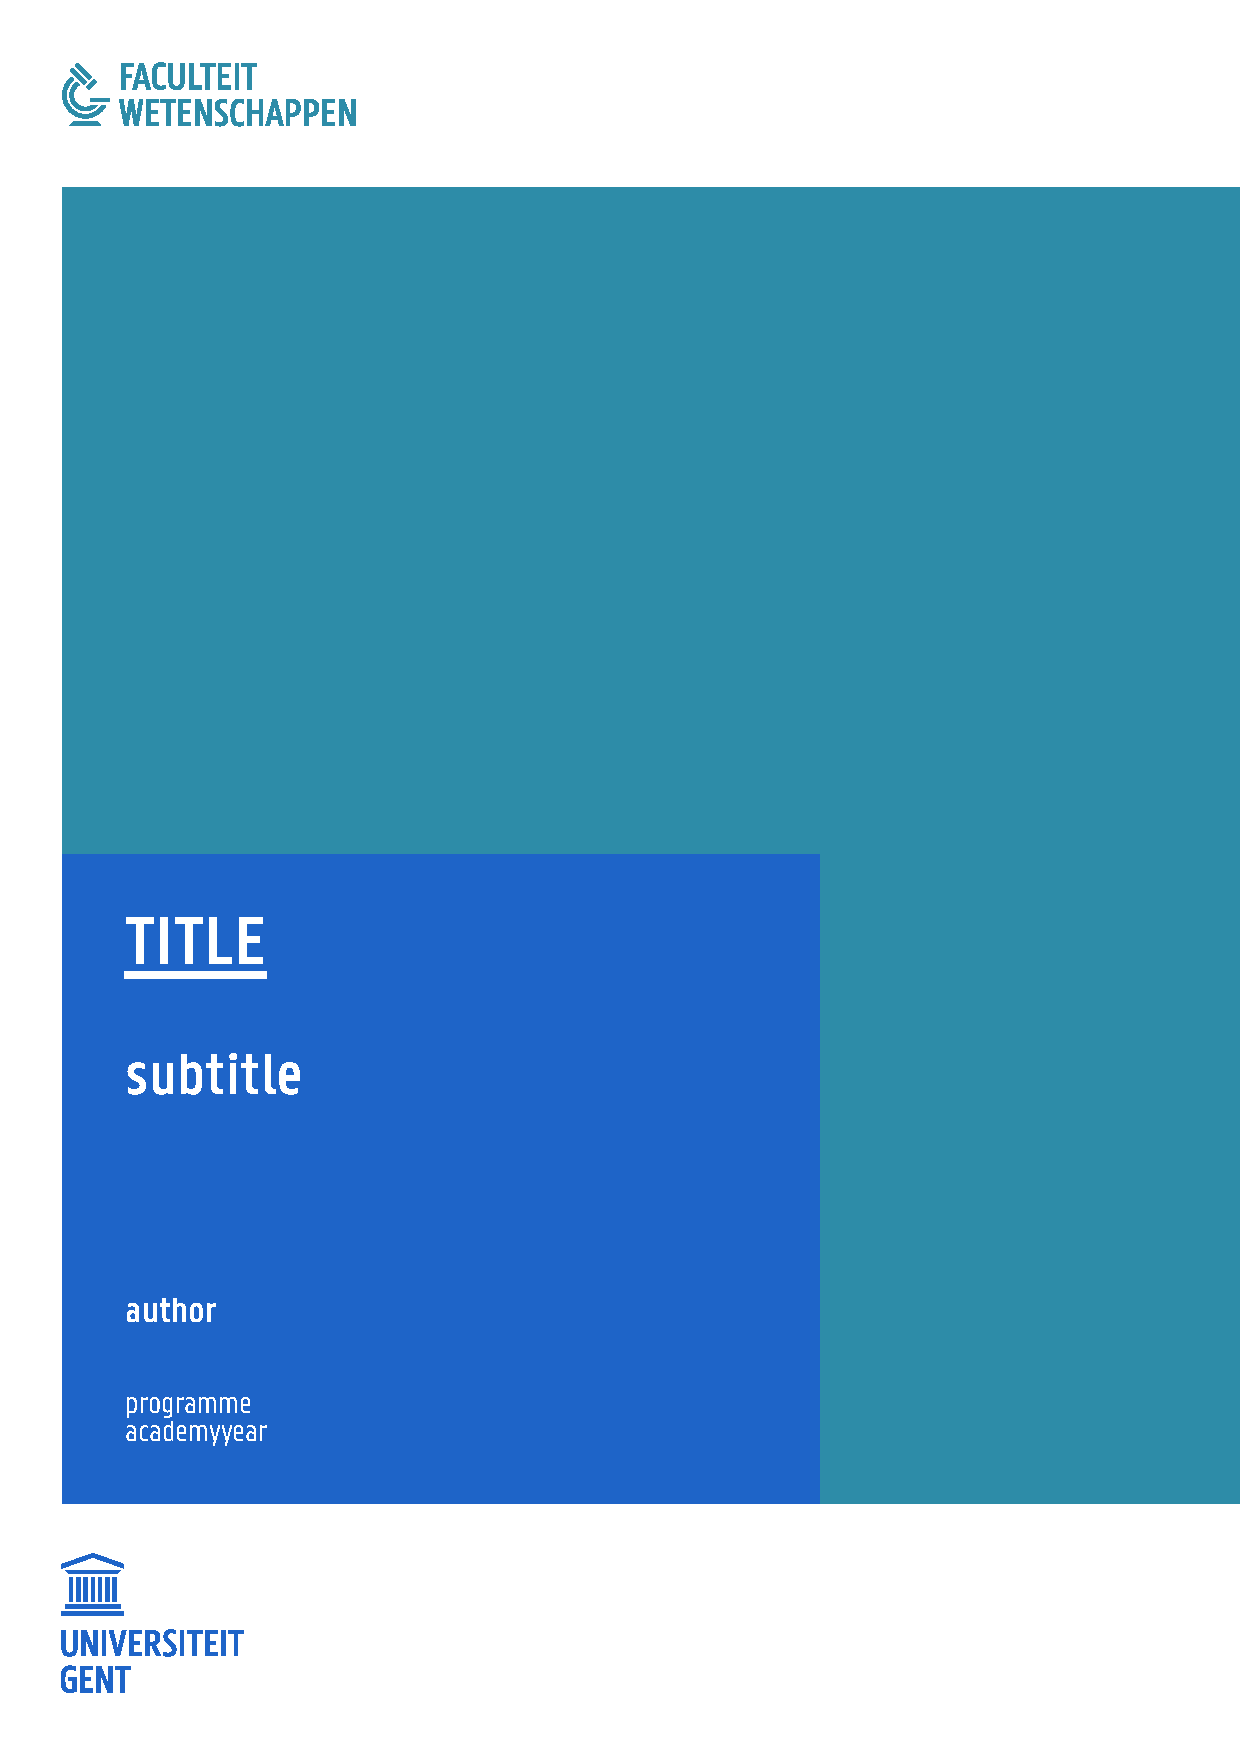
\includegraphics[width=1\textwidth]{ugent2016-title-course.pdf}}
    \end{center}

    \section{Title page type \texttt{report}}\label{sec:voorblad-met-stijl-report}
    \begin{center}
        \frame{
\includegraphics[width=1\textwidth]{ugent2016-title-report.pdf}}
    \end{center}

    \section{Title page type \texttt{notes}}\label{sec:voorblad-met-stijl-notes}
    \begin{center}
        \frame{
\includegraphics[width=1\textwidth]{ugent2016-title-notes.pdf}}
    \end{center}

    \section{Changes}\label{sec:changes}

    Changes are tracked on GitHub.

\end{document}
